\section{Análisis de la complejidad del problema}

El problema planteado por Scaloni es un caso específico del problema del 
Hitting-Set, cuya definición formal se presenta de la siguiente manera: dado un 
conjunto $A$ compuesto por $n$ elementos y $m$ subconjuntos $B_{1}, B_{2}, \dots, B_{m}$ 
pertenecientes a $A$ ($B_{i}\subseteq A \forall i \in \mathbb{N}_{m}$), se busca encontrar un conjunto $C \subseteq A$ tal que para cada 
subconjunto $C$, donde $C \subseteq A / \forall j \in \mathbb{N}_{m},  C \cap B_{j}\neq \emptyset$. 

Además de su formulación básica, el problema del Hitting-Set también presenta una versión
de decisión: dada la colección de un conjunto $A$ con $n$ elementos y $m$ subconjuntos
$B_{1}, B_{2}, \dots, B_{m}$ de $A$ ($B_{i}\subseteq A$ para cada $i$), junto con un 
parámetro numérico $k$, se plantea el interrogante sobre la existencia de un conjunto 
$C \subseteq A$ que cumpla con dos condiciones fundamentales:

\begin{itemize}
    \item En primer lugar, que la cardinalidad de $C$ sea menor o igual a $k$ ($\left| C \right|\leq k$) 
    \item En segundo lugar, que para cada subconjunto $B_{j}$, la intersección entre $C$ y $B_{j}$ no sea vacía ($C \cap B_{j} \neq \emptyset$) para todo $j$ perteneciente al conjunto de  números naturales hasta $m$.
\end{itemize}

El problema del Hitting-Set se sitúa en la clase de complejidad NP debido a su capacidad 
de verificación en tiempo polinomial, lo que implica una verificación eficiente de su 
solución propuesta. La verificación de la solución se reduce a confirmar dos condiciones 
fundamentales: Primero, se debe comprobar que la cardinalidad del conjunto propuesto $C$ 
es menor o igual a $k$, donde $k$ es un parámetro dado. Segundo, es necesario 
verificar que para cada conjunto $B_{j}$ dentro de una colección de subconjuntos 
$B_{1}, B_{2}, \dots, B_{m}$, $C$ contenga al menos un elemento de $B_{j}$.

Para realizar esta verificación, se llevan a cabo dos operaciones clave que definen la 
complejidad del proceso. La primera operación, relacionada con la verificación de la 
cardinalidad de $C$ ($\left| C \right|\leq k$), tiene una complejidad constante $O(1)$, 
ya que implica simplemente obtener el número de elementos en $C$ y verificar que $\left|C\right| \leq k$.

La segunda operación, que implica verificar la inclusión de al menos un elemento de $C$ 
en cada conjunto $B_{j}$, presenta una complejidad de $O(n \times m)$. Esto se debe a 
que para cada conjunto $B_{j}$ ($j$ perteneciente al conjunto de números naturales hasta 
$m$) (operación $O(m)$), se debe recorrer, en el peor de los casos, todo el conjunto $C$ 
($O(n)$) para verificar la pertenencia de al menos un elemento de este en $B_{j}$ 
(operación con complejidad $O(1)$ si tanto $B_{j}$ como $C$ se implementan como un conjunto 'set').

La clasificación del problema del Hitting-Set como NP-Completo se establece mediante la demostración
de su reducibilidad polinómica a partir de otros problemas ya catalogados como NP-Completo. 

En nuestro análisis, nos hemos propuesto abordar esta demostración de dos maneras distintas, 
empleando estrategias de reducción que ilustran la naturaleza NP-Completa del Hitting-Set Problem:

\begin{itemize}
    \item Reducción de Vertex Cover a Dominating-Set Problem -> Reducción de Dominating-Set Problem a Hitting-Set Problem.
    \item Reducción de Set Cover a Hitting-Set Problem.
\end{itemize}


Es importante destacar que la pertenencia de Vertex Cover y Set Cover a NP-Completo fue demostrada en clases anteriores.
\begin{itemize}
    \item  Vertex Cover [link]
    \item Set Cover [link]
\end{itemize}


\subsection{Reducción Vertex Cover a Dominating-Set Problem}

La reducción $\text{Vertex-Cover} \leq _{p} \text{Dominating-Set}$ consta en lo siguiente:
Dado del grafo $G$ con $n$ vértices y $m$ aristas del problema Vertex Cover, para cada par de 
vértices adyacentes $v-w$, se agregan ambos al grafo $G'$ (del problema Dominating Set) junto a 
su arista y se agrega un tercer vértice auxiliar $vw$, adyacente a los otros dos. $A$ será el 
conjunto de vértices auxiliares. 

Luego, del conjunto $V'$ de $k$ vértices solución de Dominating Set, se debe agregar a $V$ (solución de Vertex Cover) todos los vértices de $V'$ que no estén en el conjunto de auxiliares y, para cada vértice en $V' \cap A$ se agrega a $V$  cualquiera de sus adyacentes. La primera parte de la reducción es $O(m)$ y la segunda es $O(k),k \leq n$, por lo que la complejidad total es $O(m+k)$, que es polinomial.

\[\text{Vertex-Cover} \leq _{p} \text{Dominating-Set}\]

% \begin{figure}[H]
%     \centering
%     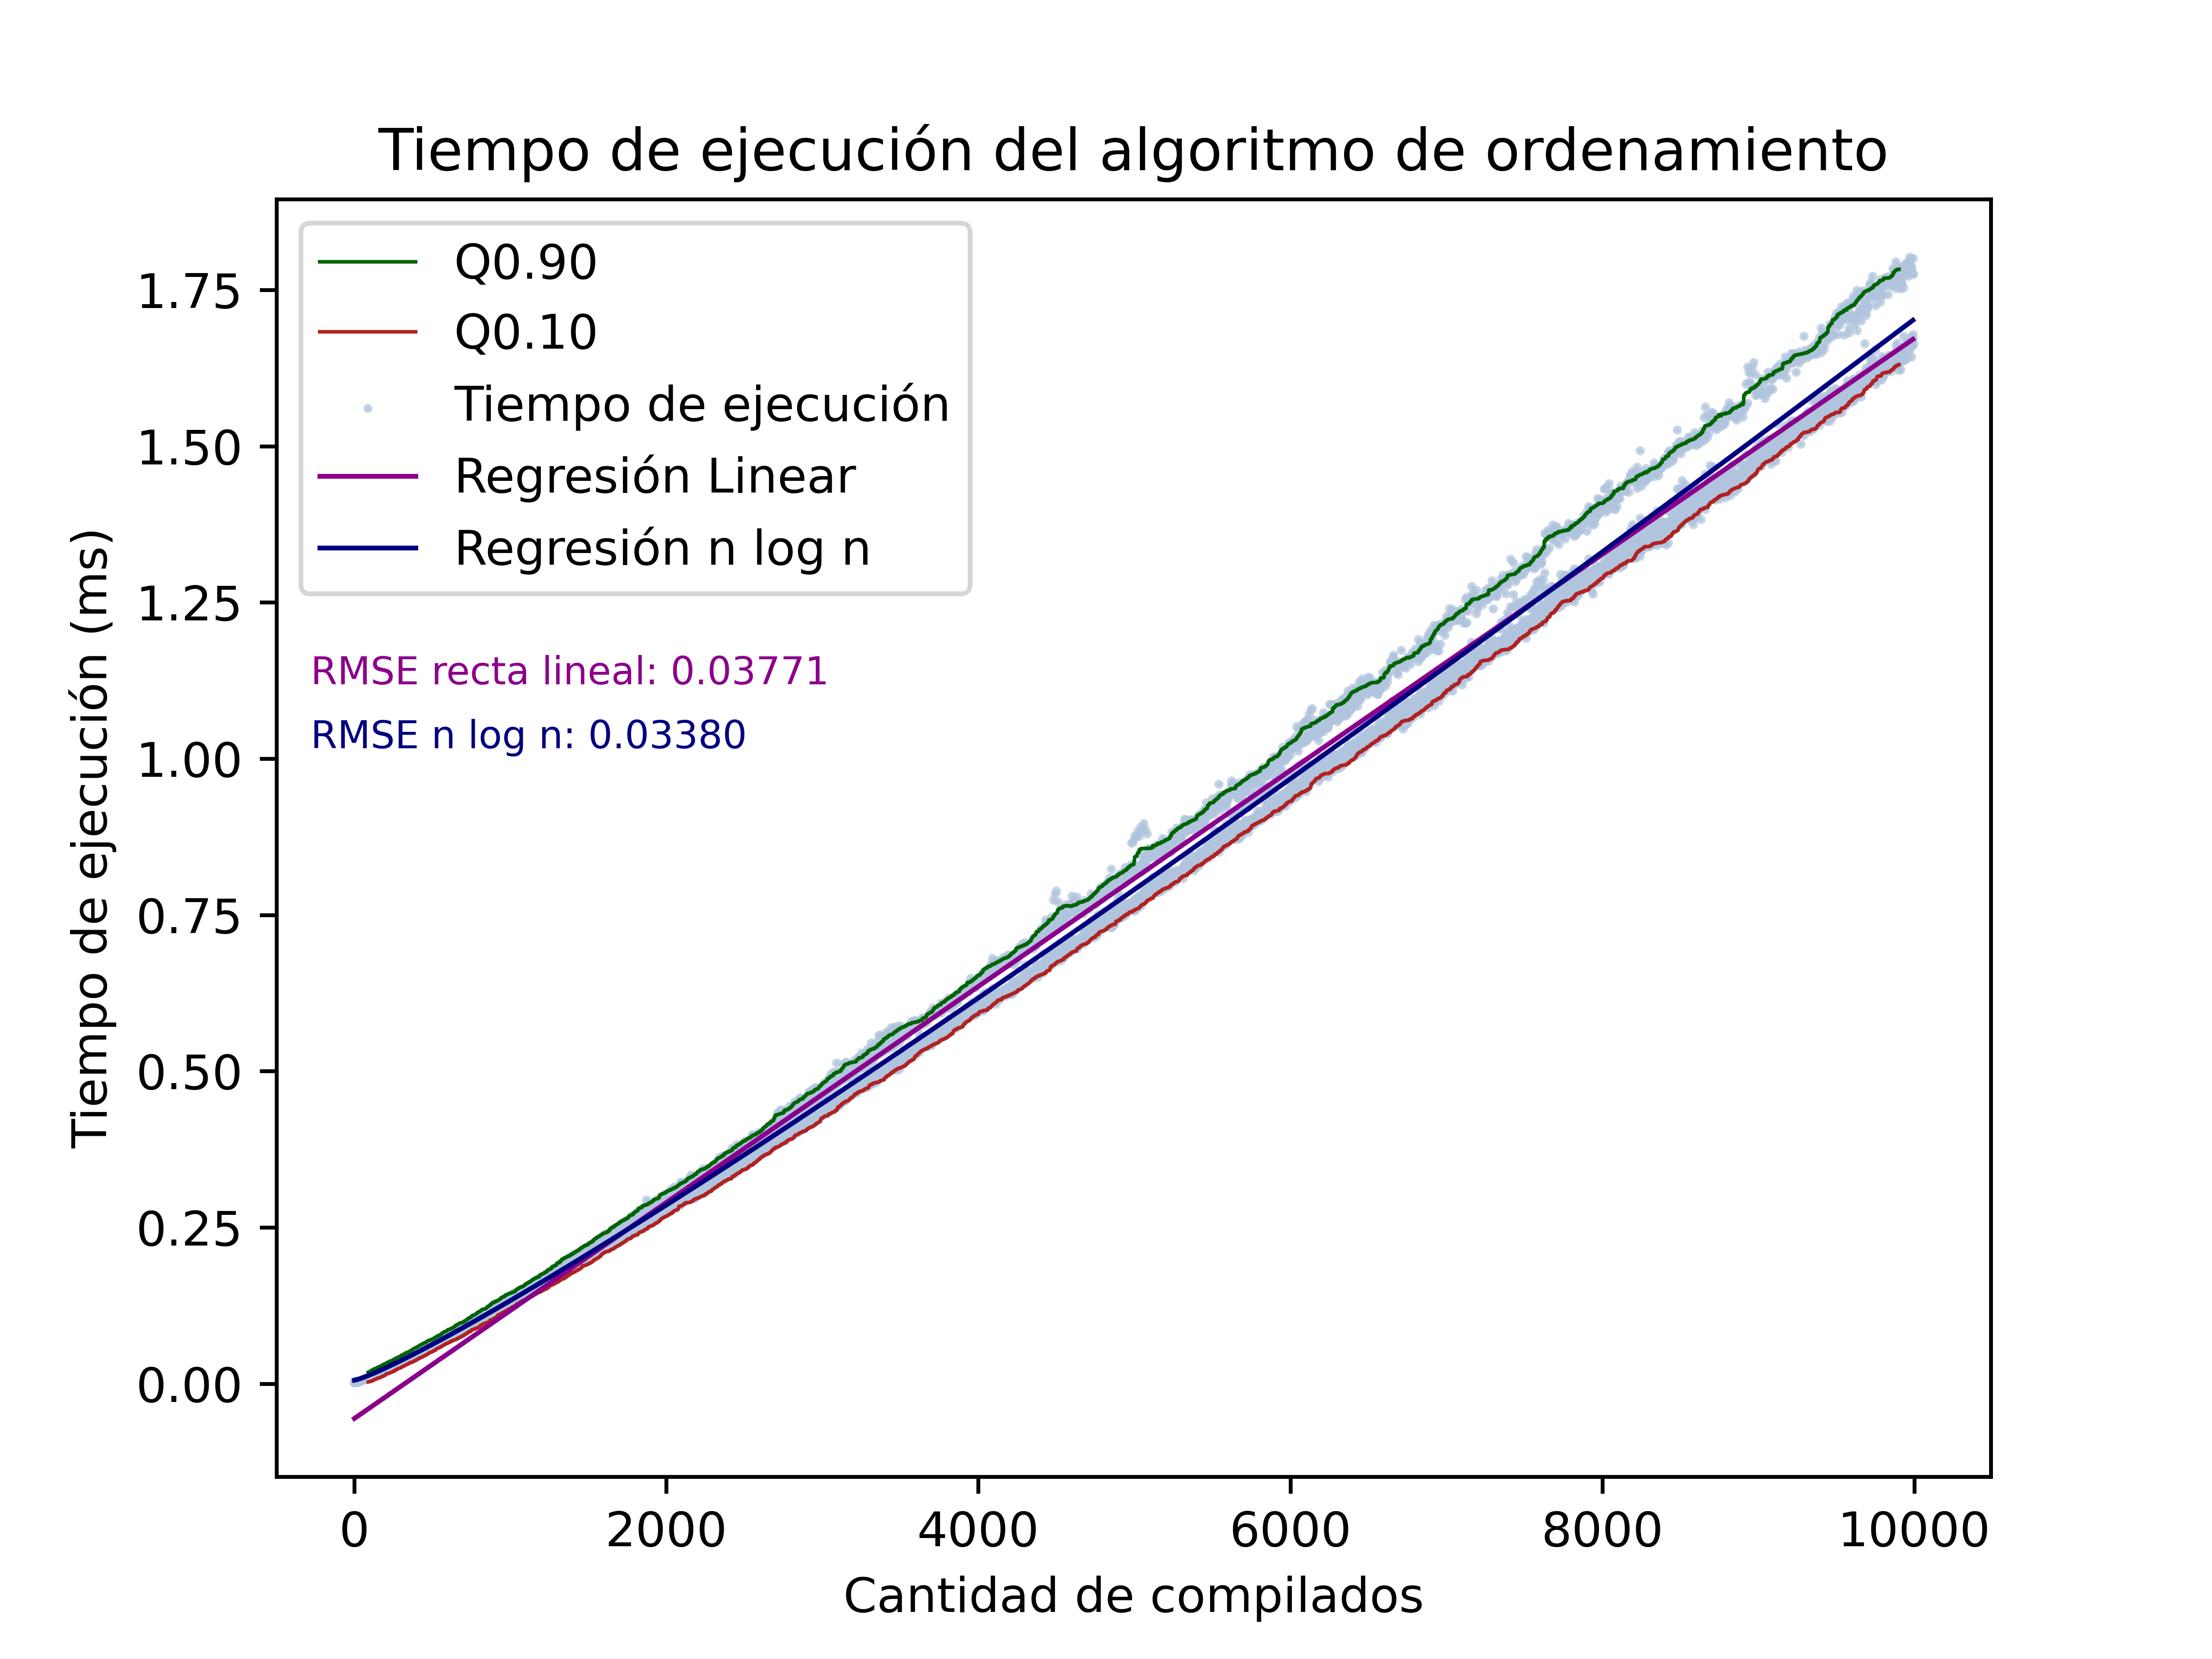
\includegraphics[width=0.8\textwidth]{img/tiempos_valores_altos_puntos.png}
%     \caption{Tendencia de la complejidad algoritmica para $n$ grandes.}
%     \label{fig:tiempos_valores_altos_puntos}
% \end{figure}

Finalmente:

\[
    \begin{array}{c}
        \begin{split}
            \text{Vertex-Cover}  & \leq _{p} \text{Dominating-Set} \\
            \text{Dominating-Set}  & \leq _{p} \text{Hitting-Set} \\
        \end{split}
        \quad \overset{ \text{por transitividad} }{ \implies  } \quad
        \text{Vertex-Cover}  \leq _{p} \text{Hitting-Set} \\ \\
        \implies \text{Hitting-Set} \in \text{NP-Completo}    
    \end{array}
\]

\subsection{Reducción Dominating-Set Problem a Hitting-Set Problem}

Recordemos el problema de Dominating Set: Dado un grafo $G$, se busca un conjunto de vértices $C$
tal que, para todo vértice $v \in G$, este esté contenido en $C$ o existe al menos un vértice en $C$ adyacente de $v$.

La reducción $\text{Dominating-Set} \leq_{p} \text{Hitting-Set}$ consta en lo siguiente:
Dado un grafo $G$ de $n$ vértices del problema Dominating Set, para cada vértice $v_{i}$, se construye un grupo $B_{i}$ con el mismo y todos sus vértices adyacentes. Entonces, el grupo resultado del Hitting Set con los subconjuntos $B_{1},B_{2},\dots,B_{m}$ será también el grupo resultado del Dominating Set. \textit{Nota: Para cada $k$-clique dentro del grafo habrá hasta $k$ sets iguales.} La complejidad de esta reducción depende de la implementación del grafo: Si los vértices desconocen a sus adyacentes, es $O(n^{2})$ porque para cada vértice $v_{i}$ se debe recorrer todos los vértices de $G$ para verificar si son adyacentes a $v_{i}$; en cambio, si los vértices tiene referencia a sus adyacentes, la complejidad es $O(n\times o)$, siendo $o$ el promedio del grado entre vértices, que puede variar entre $0$ y $m$. En ambos casos, se trata de una complejidad polinomial.

\[\text{Dominating-Set}  \leq _{p} \text{Hitting-Set}\]

% Gráficos ej de reducción

La reducción $\text{Vertex-Cover} \leq _{p} \text{Dominating-Set}$ consta en lo siguiente:
Dado del grafo $G$ con $n$ vértices y $m$ aristas del problema Vertex Cover, para cada par de vértices adyacentes $v-w$, se agregan ambos al grafo $G'$ (del problema Dominating Set) junto a su arista y se agrega un tercer vértice auxiliar $vw$, adyacente a los otros dos. $A$ será el conjunto de vértices auxiliares. Luego, del conjunto $V'$ de $k$ vértices solución de Dominating Set, se debe agregar a $V$ (solución de Vertex Cover) todos los vértices de $V'$ que no estén en el conjunto de auxiliares y, para cada vértice en $V' \cap A$ se agrega a $V$ cualquiera de sus adyacentes. La primera parte de la reducción es $O(m)$ y la segunda es $O(k),k \leq n$, por lo que la complejidad total es $O(m+k)$, que es polinomial.

\[\text{Vertex-Cover} \leq _{p} \text{Dominating-Set}\]

% Gráficos ej de reducción

Finalmente:

\[
    \begin{array}{c}
        \begin{split}
            \text{Vertex-Cover}  & \leq _{p} \text{Dominating-Set} \\
            \text{Dominating-Set}  & \leq _{p} \text{Hitting-Set} \\
        \end{split}
        \quad \overset{ \text{por transitividad} }{ \implies  } \quad
        \text{Vertex-Cover}  \leq _{p} \text{Hitting-Set} \\ \\
        \implies \text{Hitting-Set} \in \text{NP-Completo}    
    \end{array}
\]
